% !TeX root = ../main.tex
% Add the above to each chapter to make compiling the PDF easier in some editors.

\chapter{Theoretical Foundations}\label{chapter:theoreticalFoundacions}

In this chapter, we investigate the theoretical foundations by examining database performance measurements and in the next step describing used datasets and the data structure.\\We will start by discussing the characterisitcs of database systems and elaborate on the significance of performance measurements in this context. Additionally, we will outline the common performance metrics, that play a central role in the evaluation of performance analysis.
\\ For clarifying used datasets and the data structure, we commence by describing the utilized performance data, followed by giving an overview of the structure of the Benchy Viewer's input file containing the performance measurements. Moreover, the data prepration for this input file will be explained.

\section{Database Systems and Performance Measurements}
Performance measurement and analysis are fundamental in the realm of database systems. They offer valuable insights into system behavior, helping to pinpoint bottlenecks and optimization opportunities. This process is crucial not only for evaluating one's own system but also for making meaningful comparisons with other systems. Visualisations play a pivotal role in understanding performance data and are often used to convey complex findings effectively.
To interpret performance data effectively, we begin by understanding the characteristics and core traits of a Database System.

\subsection{Characteristics of Database Systems}
Database systems are complex structures that manage and store vast amounts of data efficiently, involving interrelated factors that must be finely tuned to ensure optimal performance.\\
One of the fundamental functions of a database system is query processing. A query is essentially a request for specific information from the database. This involves receiving and then executing that query. The process includes tasks like parsing, optimization, and execution.\\
Queries go through two main phases: compilation and execution. \textcolor{red}{Figure mit Compilation und Execution} During compilation, the query is transformed into an execution plan. This plan outlines the steps the system should take to retrieve the requested data. In the execution phase, the system follows this plan to fetch the data.\\
Query plans are roadmaps that guide how a database executes queries, with operators as specialized components responsible for specific actions. Operators, like selection and join operators, perform data operations during query execution, such as filtering and combining data. Optimizing query plans is vital for database efficiency, with query optimizers selecting the best plan considering factors like data distribution and hardware capabilities.\\
Query processing can be time-consuming due to various challenges. For instance, complex queries, large datasets, and suboptimal query plans can lead to slow performance. Identifying and overcoming these challenges is essential for improving system efficiency.

Understanding these characteristics is key to understanding the complexity of database performance. Challenges such as optimising query plans and dealing with large data sets are common, and manual assessment is often impractical.\\
The need for objective metrics is therefore obvious, making performance measurements essential for targeted optimisations. Due to the complexity of these metrics, visualisation techniques are invaluable for easier interpretation and analysis.\\
In the next section, we will explore the important role of performance measurements and their visualisation in improving database efficiency.


\subsection{Importance of Performance Measurements}
Database systems are the core of a wide range of applications. Consequently, their performance matters not just in terms of user-friendliness and reliability, but also in terms of efficiency. Performance measurements play a central role in this context.\\
One of the key advantages of performance measurements lies in their capacity to assist in optimization efforts. By quantifying performance in a series of metrics, database developers can pinpoint precisely where bottlenecks occur, whether it is in the compilation phase, the query plan, data retrieval, or any other component of the database system. This focused approach minimizes the trial and error often involved in performance tuning and directs resources toward the most impactful modifications.\\
Furthermore, bottlenecks and areas with room for improvement are often not obvious. With the aid of performance measurements, these elements come into sharp focus. Measurements can reveal, for example, if the system's weak point lies in query compilation or if the query plan needs to be optimized. Understanding and interpreting the findings correctly is crucial for making informed decisions on where to prioritize improvement efforts.\\
Another fundamental aspect is scalability. In a world where data is continuously growing, the scalability of a database system becomes a certain priority, because data volumes continue to grow. Performance measurements can identify the limitations of a system as it scales, revealing performance degradation points before they become critical bottlenecks. This approach is not only applied to solve current needs of data volume, but is also contributing to the system's scalability for the future.\\
Referring back to the introduction's implication, the complexity of performance metrics can often be overwhelming. Visualisation techniques become invaluable tools in this context. By translating numerical data into graphical elements, these visualisations can illuminate patterns and trends that could otherwise be easily overlooked, offering an intuitive and interactive way to understand the performance bottlenecks and operational nuances.

In summary, performance measurements are essential in the effective management and optimization of complex database systems. With these basic principles in mind, the next section examines common performance metrics for evaluating database systems, which serve as the quantitative backbone for the analyses and visualisations discussed here.

\subsection{Common Performance Metrics}
Understanding the importance of performance measurements in database systems necessitates a deeper dive into the specific metrics that help analyse various aspects of performance. This section explores effective metrics and how they are used within this domain, which indicates the desired functionalities of the Benchy Viewer in terms of interaction and visualisation.\\
In the paper "Bringing Compiling Databases to RISC Architectures" \cite{Bringin-Compiling-Databases-to-RISC} the compilation performance of the dominant x86-64 server architecture is contrasted  with the new introduced code generator designed for AArch64-based systems. This is interesting for the Benchy Viewer as it conducts a comparative analysis of different perspectives in terms of performance,  leveraging specific performance metrics that are also visually represented.\\ 
The paper utilizes both quantitative and subjective performance metrics when addressing the query compilation strategy. However, for the scope of our visualisation, we focus on the quantitative metrics. Relying on quantitative metrics allows for clear, objective visualisation that can represent performance differences, whereas subjective metrics does not offer the same level of clarity and consistency in a visual representation.\\
Here one of the most central metrics is the throughput, a key metric in databases, measures the number of processed tuples per second and is a primary optimization target. In the context of compiling databases, throughput is primarily influenced by the quality of the generated machine code for queries.\\
Another fundamental metric is the latency, which is the time needed for generating and compiling query code before execution, with lower latency being particularly important for real-time transactional systems.\\
With these two metrics, the paper shows an intuitive and clear overview of how different database instances perform on the TPC-H benchmark, as demonstrated in Figure~\ref{fig:risc-metrics}.

\begin{figure}[h]
  \centering
  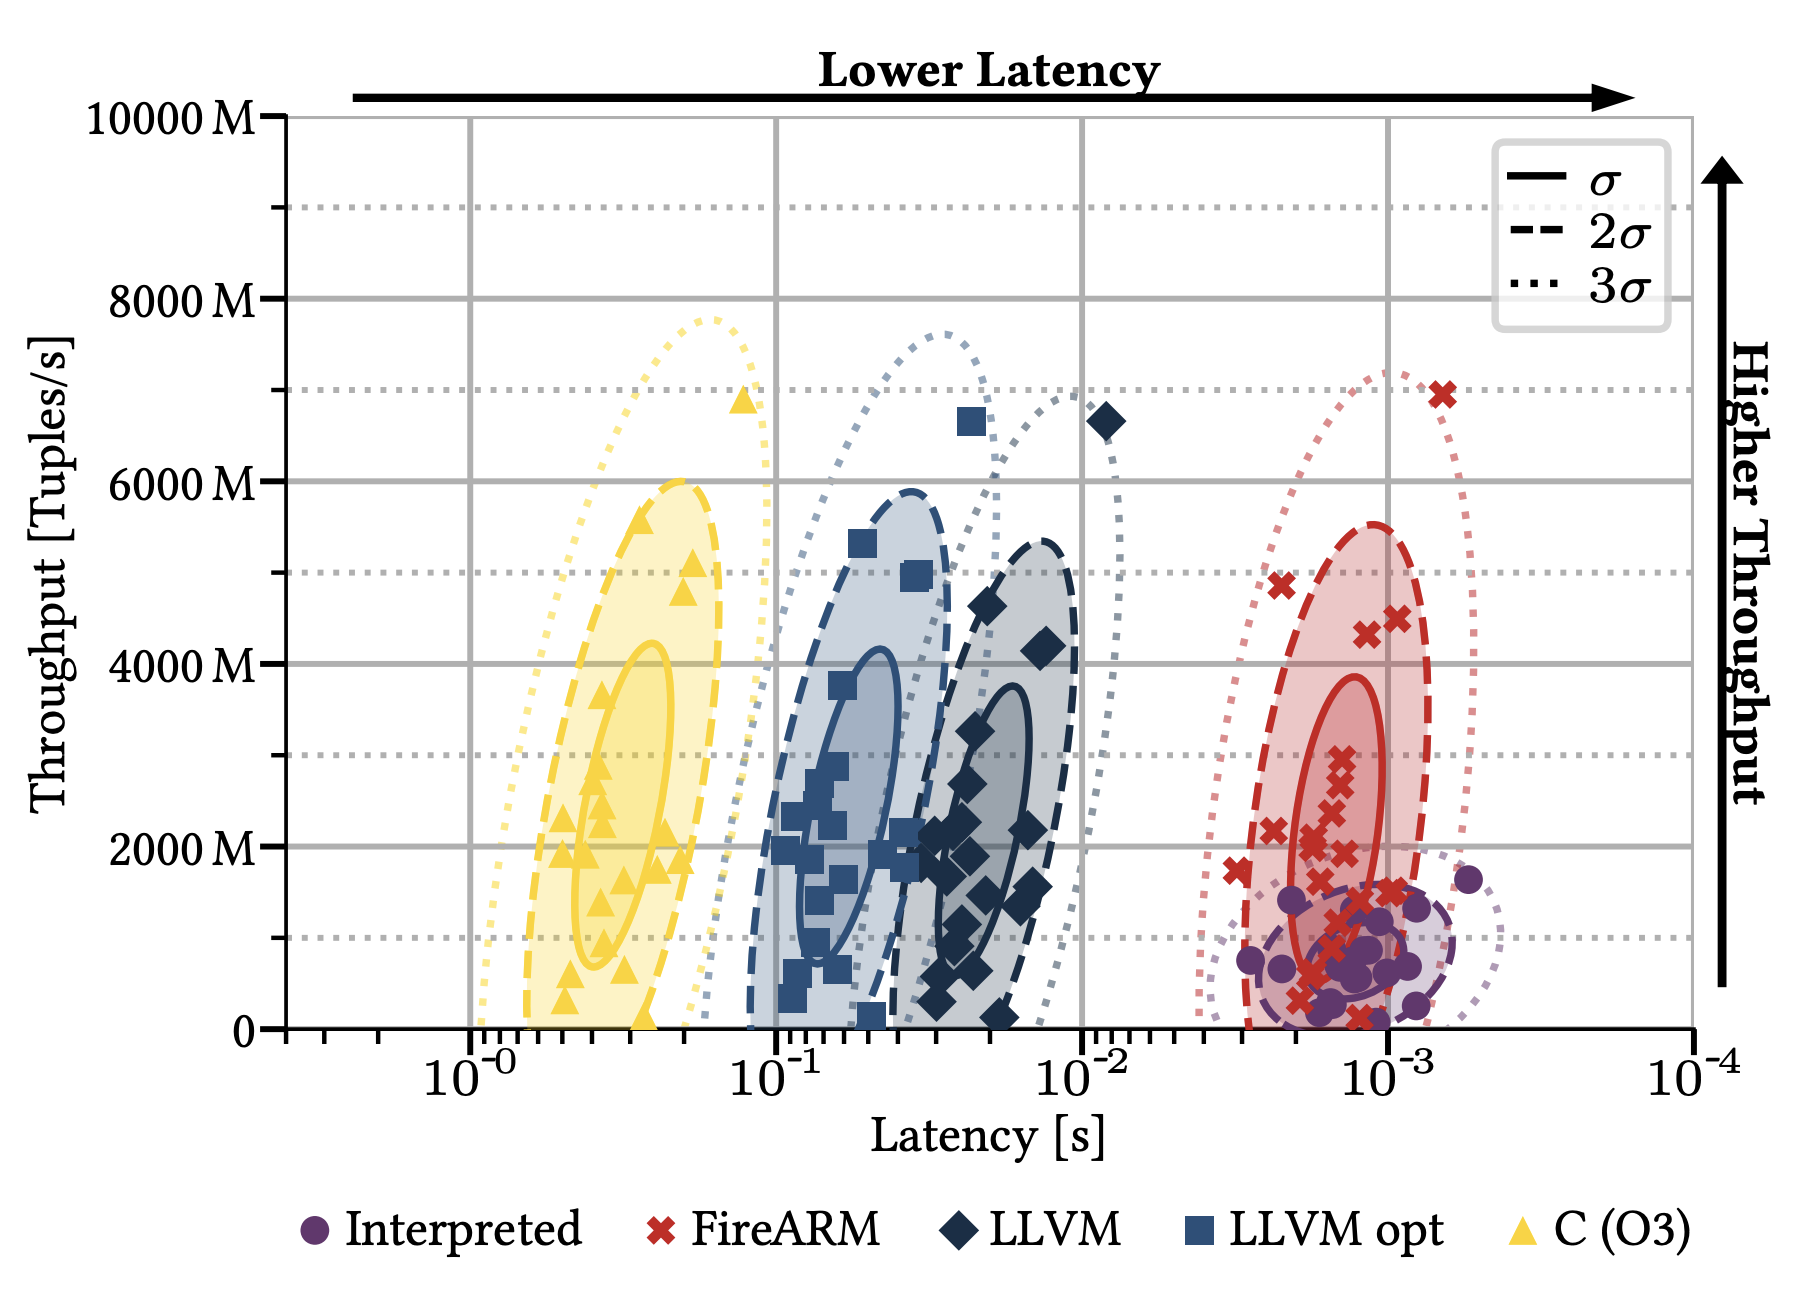
\includegraphics[width=0.8\linewidth]{figures/risc-metrcis-visualization.png}
  \caption{Visualisation example of compile-time and throughput of different query-compilation strategies running the TPC-H benchmark \cite{Bringin-Compiling-Databases-to-RISC}.}
  \label{fig:risc-metrics}
\end{figure}

\noindent

The visualisation presents a scatter plot that groups query results into clusters, with each cluster representing a database instance by a distinct color. The Y-axis displays the throughput in tuples per second, while the X-axis shows the latency in seconds, which is a descending value from left to right. Additionally, arrowed labels point to the preferred values: higher values on the Y-axis and lower on the X-axis. Thus, top-right-corner values represent optimal performance, allowing viewers to quickly identify well-performing database instances as well as the performance differences between instances.\\
In this illustration, the system highlighted in red is notable for its low latency and high throughput. Conversely, the system marked in yellow has the poorest latency performance. The instance in purple also stands out, boasting the lowest latency, but it lags behind in terms of throughput.

In the context of performance metrics, the Benchy Viewer should be capable of visualizing the key differences between instances in an intuitive and effective way. 

Besides grouping the query results into clusters, with each cluster representing a database instance, it would also be beneficial to have the flexibility to choose a specific metric for this categorization. For instance, if a database developer is primarily concerned with the metrics of execution time and throughput, they should have the option to shape the data visualisation based on these metrics.

Up next, we'll explore the dataset that is consumed by the Benchy Viewer to offer all the data and performance metrics within the analytical visualisations. We'll detail the data structure and how the data is prepared to get in this shape.

\section{Used Datasets and Data Structure}
In this section, we talk about the dataset that is consumed by the Benchy Viewer to create meaningful performance visualisations.\\
At first, we explore the diverse metrics encompassed within the dataset. For each metric, we provide a concise definition and rationalize its significance within the Benchy Viewer framework. Subsequently,  we offer an outline of the input file's structure, where we explain how database systems are mapped to the executed queries and the corresponding metric data. Finally, we describe all the steps required within the data preparation process, where raw data is transformed into the previously specified format.

\subsection{Description of the Utilized Performance Data}
In this section, we take a closer look at the performance data which is utilized by the Benchy Viewer. These data contain various metrics that give us insights into how our database system is performing: total time (compilation, execution), cycles, instructions, L1 data cache misses, LLC (Last-Level Cache) misses, branch misses, DTLB (Data Translation Lookaside Buffer) misses, tasks, instructions per cycle (IPC), CPU frequency (GHz), and scalability metrics. 

\textbf{Total time} represents the combined time taken for both query compilation and query execution. It's a critical measure of how efficiently queries are processed. Lower total times are desired, indicating faster query processing.

\textbf{Compilation} is the preparation for the execution phase where source code, written in a high-level language, is converted into a lower-level representation. Producing highly-optimized code in this stage can significantly enhance the speed and efficiency of program execution.

\textbf{Execution} refers to the phase after the compilation phase where the compiled code is executed on a CPU. It involves the actual processing of instructions and data to perform the tasks specified by the program. The execution phase is of vital significance as it directly measures how efficiently a program or task runs on the hardware.

\textbf{Instructions} count the number of individual machine-level instructions during the execution of a program or a specific operation and helps assessing the efficiency of code execution. A high instruction count indicates that the program is performing a large number of computations, which impacts CPU utilization and overall performance. Well-optimized code tends to have a lower instruction count for the same computational tasks. While instruction count provides valuable information about code complexity, it does not capture the complete performance picture. For a more comprehensive understanding, it should be considered alongside metrics such as cycle counts and IPC (Instructions Per Cycle).

\textbf{Cycles} refer to the number of clock cycles executed during the test by a CPU. It measures the raw computational effort involved and can indicate the CPU's workload. Lower cycle counts indicate more efficient code execution, while higher counts suggest greater computational complexity or inefficiencies. While cycles provide valuable information about computational effort, they do not give a complete picture of overall system performance. Other metrics, such as instructions per cycle (IPC), may be necessary to better understand the performance landscape.

\textbf{IPC (Instructions Per Cycle)} is a performance metric that measures the average number of instructions during a single clock cycle. A higher IPC value indicates that the CPU is executing more instructions per clock cycle, which suggests better performance. Well-optimized code and algorithms tend to have higher IPC values.

\textbf{L1D-Misses (Level 1 Data Cache Misses)} are a performance metric that counts the number of times a CPU requested data from its Level 1 Data Cache but was unable to find the required data there. Instead, the CPU had to retrieve the data from a higher-level cache or main memory. The number of L1D-Misses is significant because it reflects how efficiently the CPU's cache hierarchy is operating. High L1D-Miss rates suggest that the CPU frequently needs to access data from slower memory levels, resulting in increased latency and potentially impacting overall system performance. Lower L1D-Miss rates generally indicate more efficient cache utilization and can result in improved execution performance.

\textbf{LLC-Misses (Last-Level Cache Misses)} are a performance metric that counts the number of times a CPU failed to find requested data in its last-level cache. Instead, it had to retrieve the data from a slower memory hierarchy level, such as a higher-level cache or main memory. The number of LLC-Misses is significant because it indicates how effectively the CPU's last-level cache is utilized. Similar to L1D-Misses high LLC-Miss rates suggest that frequently accessed data is not readily available in the cache, leading to increased memory access latency and potential performance bottlenecks. Lower LLC-Miss rates generally indicate more efficient cache utilization and can lead to better overall execution performance.

\textbf{Branch-Misses}, often referred to as "branch mispredictions," are a performance metric that counts the number of times a CPU incorrectly predicts the outcome of a branch instruction. Branch instructions are conditional statements (e.g., if-else or loops) in code that determine the program's flow based on a condition. A branch miss occurs when the CPU's branch predictor guesses incorrectly about the branch's outcome and, as a result, has to discard or re-execute some instructions. Therefore, high Branch-Miss rates can indicate inefficiencies in the code execution, as mispredicted branches can lead to the execution of unnecessary instructions and decreased overall performance. Several factors influence Branch-Miss rates, including the complexity of code logic, the CPU's branch prediction algorithms, and the effectiveness of compiler optimizations. Other metrics, such as instruction count, cycle count, and cache utilization, should be also considered to obtain a comprehensive view of performance.

\textbf{DTLB-Misses (Data Translation Lookaside Buffer Misses)} are the number of times a CPU requested data from memory, and during this request, it also needed to fetch or translate the virtual memory address to its corresponding physical memory address, but couldn't find the translation in the Data Translation Lookaside Buffer (DTLB). Instead, it had to consult a more extensive translation structure, such as the page table in memory, to perform the translation. The number of DTLB-Misses is significant because it indicates how effectively the CPU's DTLB, which is responsible for accelerating memory address translation, is functioning. High DTLB-Miss rates suggest that the translation process is less efficient, leading to increased memory access latency.

\textbf{Tasks} refer to concurrent units of work or threads that a computer system or application is managing or executing simultaneously. These tasks may represent various processes, threads, or parallel workloads. The number of tasks and their management is significant because it reflects the system's concurrency and workload handling capacity. They help assess how well a system scales with increased workloads and concurrent tasks.

\textbf{CPUs} are defined by the number of cores utilized by the system. A higher number of CPUs implies a higher degree of concurrent computing, potentially leading to executing the given query in a more efficient manner. However, the effectiveness of parallel processing also depends on factors like architecture, clock speed, and the specific nature of the computing tasks.

\textbf{GHz (Gigahertz)} is a unit of measurement used to quantify the clock speed or frequency of a CPU or other electronic components within a computer system. Specifically, it represents one billion cycles per second. In computing, it is primarily used to describe the operating frequency of a CPU. The GHz metric is significant because it reflects how quickly a CPU can process instructions and perform calculations. Higher GHz values generally indicate faster processing speeds, which can lead to quicker execution of tasks and improved system performance.

\textbf{Scale}, in the context of performance analysis for databases, refers to the size of the dataset. It quantifies the system's ability to handle increasing amounts of data and workload. Scale is often measured in terms of data volume, storage capacity, or concurrent user connections. Scale-related metrics are essential for benchmarking and comparing different database systems, hardware configurations, or software designs. They help assess how systems perform as data or workload sizes increase and enable informed decisions regarding system scalability.

In this section, we have provided a comprehensive overview of the performance metrics that will be employed in our system. The next section will detail how we format and organize our performance data for analysis.



\subsection{Structure of the Input File with Performance Measurements}\label{sec:input-file-structure}
One step preceding the utilization of the Benchy Viewer is the provision of the benchmark data, which will be later used to generate the performance visualisations. In this section, we give an overview about the structure of the input file for the Benchy Viewer.

When submitting data to the Benchy Viewer, only one CSV file is needed to be uploaded to the system. This CSV file contains the benchmark data of all the participating database systems.

\begin{figure}[h]
  \centering
  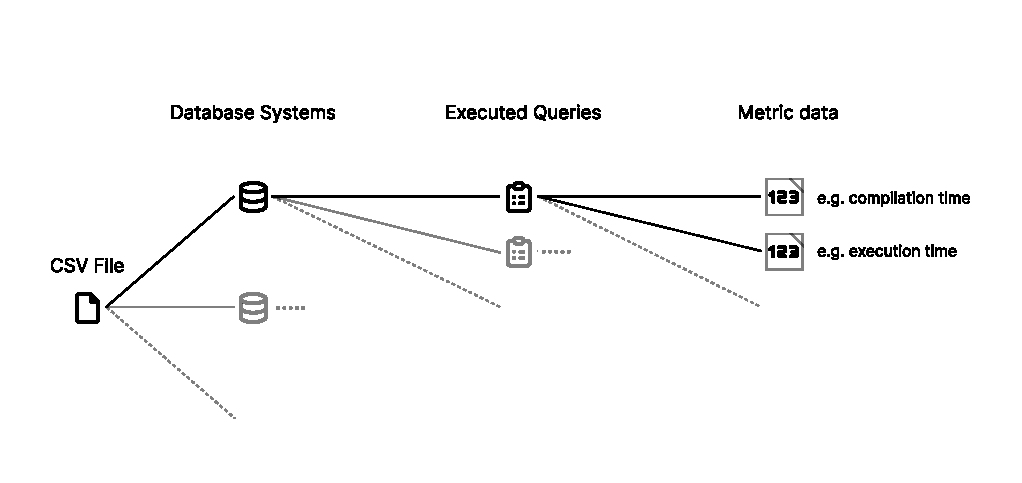
\includegraphics[width=1\linewidth]{figures/csv-structure.pdf}
  \caption{CSV structure of the input data for the Benchy Viewer}
  \label{fig:csv-structure}
\end{figure}

The structure of the input file, as depicted in Figure~\ref{fig:csv-structure}, is well-defined. It contains the entries of the respective database systems, with each query being associated with a database system. For example, when comparing TPC-H benchmark data, each database should comprise data for all 22 TPC-H queries. Each individual query contains data for multiple metrics, which were defined in the previous section such as compilation time, execution time, cycles, instructions, etc.

Moreover, the system accommodates the use of multiple instances of a single database system. Within a database system entry, there is an attribute that allows the specification of the system's particular version. Besides, comparing different systems, this feature enables the comparison of different configurations within one system.

The queries contain metric data  which are expressed in specific units or data types. Time-related metrics, such as total, compilation, and execution times, are measured in milliseconds, offering insights into the temporal aspects of query processing.\\
Hardware-related metrics, including cycles, instructions, cache misses, and more, are provided as integer values, reflecting various hardware-level details. Task-related metrics are also presented as integers, helping to assess task-specific performance. IPC metrics are in floating-point numbers, offering a nuanced perspective on instruction efficiency. CPU-related metrics are integers, while frequency-related metrics are in gigahertz (GHz), providing information about CPU clock speeds.

Next up is the "Data Preparation" section, where we'll dive into the necessary steps for formatting and structuring our data to make it compatible with the Benchy Viewer.

\subsection{Data Preparation}
Prozess, wie man die Daten von einem Testdurchlauf bekommt und davon ein CSV erstellt
-> Max fragen

